\chapter{Introduction}
\label{ch:intro}
\section{Shock-Capturing Schemes}

Hyperbolic partial differential equations (PDE) allow for both smooth and discontinuous solutions. A system of hyperbolic PDEs that are of particular interest in computational fluid dynamics of compressible flows are the Euler equations. The Euler equations are a simplification of the Navier-Stokes equations and govern the physics of inviscid fluid flow. The solutions of one-dimensional Euler equations allow for three types of waves --- rarefactions, contact discontinuities, and shock waves. The latter two waves contain strong discontinuities and regions of high gradients that pose a problem for the classical Finite Volume Method (FVM). In computational fluid dynamics (CFD), two approaches exist to increase the accuracy at regions with high gradients. Shock-fitting schemes employ a moving grid or shock-tracking to increase the order of accuracy. In either case, the shock-fitting schemes require prior knowledge of the discontinuity to increase the order of accuracy. Shock-capturing schemes employ several techniques to increase the solution's accuracy near high gradients that do not require prior knowledge of the discontinuity. The majority of shock-capturing methods are first-order and give rise to spurious oscillations near discontinuities. Many shock-capturing methods attempt to preserve monotonicity by the addition of numerical diffusion near discontinuities. In this study, an alternative approach to increasing the order of the Roe approximate Riemann solver is investigated using higher-order reconstruction or the modification of the average flux term in Roe's formulation for the cell-face fluxes.

Well-known shock-capturing methods include the MacCormack scheme \cite{MACCORMACK2003405}, higher-order finite-difference total variation diminishing (TVD) methods introduced by Harten \cite{HARTEN1983357}, the van Leer scheme \cite{VANLEER1997}, and Riemann solvers. The MacCormack scheme is a two-step extension of the Lax-Wendroff \cite{LAXWENDROFF1960132} scheme. The MacCormack and Lax-Wendroff schemes are both second-order finite difference methods; however, the MacCormack scheme uses a predictor and a corrector step, in which one step is a forward difference and the other is a backward difference. The TVD schemes of Harten ensure monotonicity by the addition of numerical viscosity to the solution by way of a viscosity function. The van Leer scheme was a correction to the Steger-Warming \cite{STEGER1981263} flux-splitting scheme in which the flux is split into two subvectors consisting of those associated with the positive eigenvalues and the negative eigenvalues of the Jacobian matrix. The van Leer scheme addresses the issues that arise in transonic regions in the Steger-Warming scheme by taking the flux's value as the summation of the split fluxes in transonic and subsonic regions. Riemann solvers take advantage of the fact that the discontinuity between the left and right states is similar to the Riemann problem and solve the Riemann problem for the intercell flux.

Godunov \cite{godunov:hal-01620642} is credited with the first exact Riemann solver. Godunov proposed a scheme that computed the solution to the Riemann problem at the cell interface. Godunov used a constant piecewise, cell-centered extrapolation of the data to represent the Riemann problem at the cell face. Godunov's method then solves the initial value problem (IVP) for the conservation laws using the data's constant piecewise representation. Solving the IVP leads to local Riemann problems at the intercell face positions. Godunov's method then solves the local Riemann problem exactly. However, the exact solution for pressure in the local Riemann problem requires an iterative method to solve the pressure function. Solving the Riemann problem approximately can avoid this iterative method to find the pressure.

Approximate Riemann solvers are a class of shock-capturing schemes that approximate the analytic solution to the Riemann problem.  Many approximate Riemann solvers have been developed.  The Harten-Lax-van Leer (HLL) \cite{HARTENLAXVANLEER1983251} solver uses a two-wave approach that assumes the solution consists of two waves separating three regions of constant data. This assumption is only correct for hyperbolic systems containing two equations, such as the shallow water equations. The Harten-Lax-van Leer-Contact (HLLC) solver of Toro, Spruce, and Speares \cite{TOROSPRUCESPEARES199441} extends the HLL solver to three-wave systems such as the Euler equations by restoring the contact surface. Roe \cite{ROE1997250} proposed an approximate Riemann solver based on the linearized Jacobian that uses a Roe-averaged matrix that is then solved exactly to compute the interface flux. Roe's method uses the eigenvalues and eigenvectors of the linearized Jacobian to directly solve for the wave strengths. The Roe flux consists of two terms --- an average flux and a diffusive flux. The diffusive flux uses the wave strengths, eigenvalues, and eigenvectors, while the average flux consists of the simple average of the left and right fluxes. Most methods to increase Roe's solver's order involve higher-order reconstruction of the left and right states. This study considers two approaches to increase the order of Roe's solver. The first approach uses higher order reconstruction of the left and right states at an interface, which are then used both in the average and diffusive fluxes. The second approach retains the higher order reconstruction of the first approach for the diffusive flux but employs higher order central differencing based on the conserved variables at the cell centers for the average flux.

There have been many improvements to Roe's approximate Riemann solver. Roe and Pike \cite{ROEPIKE1985} introduced a refinement to the method that does not require calculating the Roe-averaged matrix. Roe and Pike introduced a Roe-Pike-averaged vector of primitive variables, which can be used to evaluate the wave strengths directly. Glaister \cite{GLAISTER1988382,GLAISTER1988361} used the Roe-Pike method to extend Roe's solver to the time-dependent Euler equations and the three-dimensional Euler equations. Roe \cite{ROE1992132} introduced a sonic fix in which the numerical flux is modified at the sonic point and both the neighboring cell faces. Einfeldt, Munz, Roe, and Sjögreen \cite{EINFELDT1991273} introduced corrections to avoid the vacuum problem near low densities. This correction consisted of splitting the signal speeds and adding an anti-diffusion coefficient that guaranteed positive densities and pressures. 

Shocks and contact waves are discontinuous, and the Riemann problem provides a good approximation for these types of waves. Rarefactions, however, involve a continuous change in variables, and the linearized approximation across data jumps can be misrepresented and lead to unphysical, entropy violating, rarefaction shocks.  Dubois and Mehlman \cite{DUBOISMEHLMAN1993311} and Harten and Hyman \cite{HARTEN1983235} introduced corrections to avoid the appearance of rarefaction shocks. Dubois and Mehlman modified the flux function to include a unique Hermite polynomial that gives Roe's flux at non-sonic points but corrects the data's misrepresentation at sonic points. This thesis makes use of Harten and Hyman's approach to the entropy fix. The Harten-Hyman entropy fix calculates new wave speeds in the cases of transonic rarefactions using the velocity and speed of sound in the regions between the left and right states and uses these newly corrected wave speeds in the calculation of the flux.

van Leer \cite{VANLEER1979101} produced the first high-order TVD scheme by replacing Godunov's piecewise constant approximation with a piecewise linear approximation. The Monotonic Upwind Scheme for Conservation Laws (MUSCL) achieved second-order accuracy by reconstructing the left and right states and limiting their gradients. The flux limiter function ensures that the reconstruction is first-order in regions of high gradients and second-order in smooth regions. In this study, the second-order MUSCL reconstruction is used as a comparison against the third and fifth-order WENO reconstructions. The effects of higher-order central differencing on the average flux along with MUSCL reconstruction of the diffusive flux are also investigated.

Harten and Osher \cite{HARTENOSHER1987279} refined the idea of replacing the piecewise constant approximation with the introduction of Essentially Non-Oscillatory (ENO) schemes. Harten, Engquist, Osher, and Chakravarthy \cite{HARTEN19973} completed the ENO schemes and the stencil selection process. ENO schemes compare reconstruction polynomials and choose the smoothest of the polynomials so that a piecewise linear reconstruction is recovered that omits cells from the stencil that include discontinuities. The stencil selection process for the ENO scheme involves many conditional statements that are cumbersome for computations. Liu, Osher, and Chan \cite{LIU1994200} developed new Weighted ENO (WENO) schemes that avoid the stencil selection process by adaptively excluding the discontinuous cell. The WENO schemes choose a convex combination of all the stencils and assign nonlinear weights such that the stencil containing the discontinuous cell is assigned a zero or almost zero weight. Jiang and Shu \cite{1996JCoPh.126..202J} then proposed new smoothness measurements that were more accurate at critical points than the WENO schemes of Liu, Ohser, and Chan. Jiang and Shu's smoothness measurements made use of the sum of the $L^2$ norms of the derivatives of the interpolating polynomial, rather than the total variation $L^1$ based smoothness measurement. This development led to smoother, more accurate stencils. In the higher-order reconstruction approach and the higher-order reconstruction with higher-order central differencing approach, this thesis uses a third and fifth-order WENO reconstruction with Jiang and Shu's improved smoothness indicators to extend Roe's scheme to higher-order.

\section{Approach}

%\tikzstyle{decision} = [diamond, draw, fill=blue!50, 
%text width=4.5em, text badly centered, node distance=3cm, inner sep=0pt]
%\tikzstyle{block} = [rectangle, draw, fill=blue!20, 
%text width=5em, text centered, rounded corners, minimum height=4em]
%\tikzstyle{line} = [draw, -latex']
%\tikzstyle{cloud} = [draw, ellipse,fill=red!20, node distance=3cm,
%minimum height=2em]

\tikzstyle{reconstruction} = [rectangle, minimum width=0.5cm, minimum height=0.5cm, text centered, draw=black, fill=green!30]
\tikzstyle{RoeFlux} = [rectangle, minimum width=0.5cm, minimum height=0.5cm, text centered, draw=black, fill=orange!30]
\tikzstyle{Flux} = [rectangle, minimum width=0.5cm, minimum height=0.5cm, text centered, draw=black, fill=blue!30]
\tikzstyle{CDFlux} = [rectangle, minimum width=0.5cm, minimum height=0.5cm, text centered, draw=black, fill=red!30]
\tikzstyle{HORCD} = [rectangle, minimum width=0.5cm, minimum height=0.5cm, text centered, draw=black, fill=black!30]
\tikzstyle{line} = [draw, thick]

%\begin{figure}
%	\centering
%	\begin{tikzpicture}[node distance=2cm]
%		\node[align=center] (roeflux) [RoeFlux] {Roe Flux \\ $\boldsymbol{F}_{i+\frac{1}{2}} = \frac{1}{2} \left( \boldsymbol{F}_L + \boldsymbol{F}_R \right)- \frac{1}{2}\sum_{i = 1}^{m} \tilde{\alpha}_i  |\tilde{\lambda}_i |  \tilde{\boldsymbol{K}}^{\left(i\right)}$};
%		\node[align=center] (AvgFlux) [Flux, below of=roeflux, xshift=-7em] {Average Flux \\ $\frac{1}{2} \left( \boldsymbol{F}_L + \boldsymbol{F}_R \right)$};
%		\node[align=center] (DiffFlux) [Flux, below of=roeflux, xshift=7em] {Diffusive Flux \\ $\frac{1}{2}\sum_{i = 1}^{m} \tilde{\alpha}_i  |\tilde{\lambda}_i |  \tilde{\boldsymbol{K}}^{\left(i\right)}$};
%		\node[align=center] (Interface) [CDFlux, below of=AvgFlux, xshift=-4em] {Cell Interface \\ $\frac{1}{2} \left( \boldsymbol{F}_L + \boldsymbol{F}_R \right)$};
%		\node[align=center] (CellCenter) [CDFlux, below of=AvgFlux, xshift=5.5em] {Cell Center \\ $\frac{1}{2} \left( \boldsymbol{F}_{i} + \boldsymbol{F}_{i+1} \right)$};
%		\node[align=center] (Roe1) [reconstruction, below of=Interface,xshift=-3.89em,yshift=1em] {\tiny Roe};
%		\node[align=center] (MUSCL1) [reconstruction, below of=Interface,xshift=-1.5em,yshift=1em] {\tiny MUSCL};
%		\node[align=center] (WENO31) [reconstruction, below of=Interface,xshift=1.5em,yshift=1em] {\tiny WENO3};
%		\node[align=center] (WENO51) [reconstruction, below of=Interface,xshift=4.54em,yshift=1em] {\tiny WENO5};
%		\node[align=center] (Roe2) [reconstruction, below of=DiffFlux, xshift=-3.89em,yshift=1em] {\tiny Roe};
%		\node[align=center] (MUSCL2) [reconstruction, below of=DiffFlux, xshift=-1.5em,yshift=1em] {\tiny MUSCL};
%		\node[align=center] (WENO32) [reconstruction, below of=DiffFlux, xshift=1.5em,yshift=1em] {\tiny WENO3};
%		\node[align=center] (WENO52) [reconstruction, below of=DiffFlux, xshift=4.54em,yshift=1em] {\tiny WENO5};
%		\node[align=center] (CD2) [HORCD, below of=CellCenter, xshift=-2em,yshift=1em] {\tiny CD2};
%		\node[align=center] (CD4) [HORCD, below of=CellCenter,yshift=1em] {\tiny CD4};
%		\node[align=center] (CD6) [HORCD, below of=CellCenter, xshift=2em,yshift=1em] {\tiny CD6};
%		
%		\path[line] (roeflux.south) -- + (0,-1em) -| (AvgFlux);
%		\path[line] (roeflux.south) -- + (0,-1em) -| (DiffFlux);
%		\path[line] (AvgFlux.south) -- + (0,-1em) -| (Interface);
%		\path[line] (AvgFlux.south) -- + (0,-1em) -| (CellCenter);
%		\path[line] (DiffFlux.south) -- + (0,-1em) -| (Roe2);
%		\path[line] (DiffFlux.south) -- + (0,-1em) -| (MUSCL2);
%		\path[line] (DiffFlux.south) -- + (0,-1em) -| (WENO32);
%		\path[line] (DiffFlux.south) -- + (0,-1em) -| (WENO52);
%		\path[line] (Interface.south) -- + (0,-1em) -| (Roe1);
%		\path[line] (Interface.south) -- + (0,-1em) -| (MUSCL1);
%		\path[line] (Interface.south) -- + (0,-1em) -| (WENO31);
%		\path[line] (Interface.south) -- + (0,-1em) -| (WENO51);
%		\path[line] (CellCenter.south) -- + (0,-1em) -| (CD2);
%		\path[line] (CellCenter.south) -- + (0,-1em) -| (CD4);
%		\path[line] (CellCenter.south) -- + (0,-1em) -| (CD6);
%	\end{tikzpicture}
%	\caption[Roe Flux Calculation Outline]{Roe Flux Calculation Outline}
%	\label{fig:RoeFluxFlowChart}
%\end{figure}

\begin{figure}
	\centering
	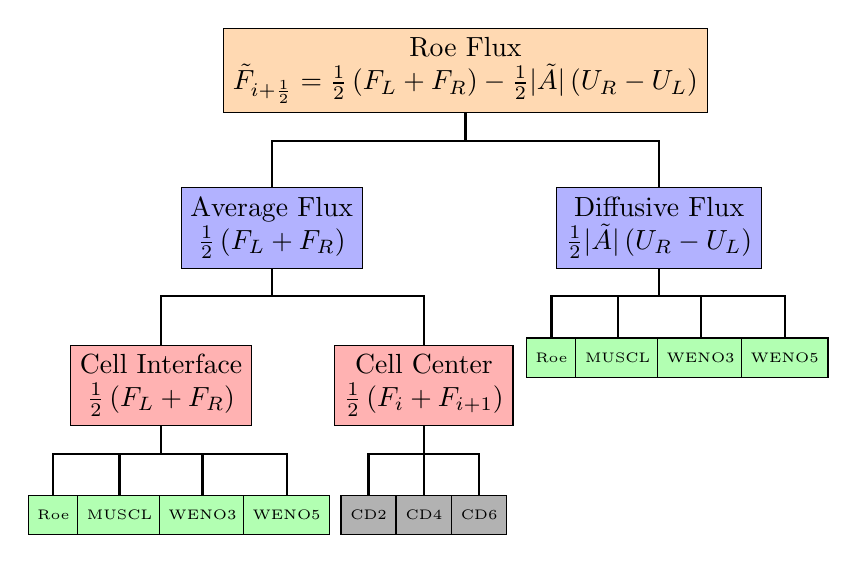
\begin{tikzpicture}[node distance=2cm]
		\node[align=center] (roeflux) [RoeFlux] {Roe Flux \\ $\boldsymbol{\tilde{F}}_{i+\frac{1}{2}} = \frac{1}{2}\left(\boldsymbol{F}_L + \boldsymbol{F}_R\right) - \frac{1}{2} |\boldsymbol{\tilde{A}}| \left(\boldsymbol{U}_R - \boldsymbol{U}_L\right)$};
		\node[align=center] (AvgFlux) [Flux, below of=roeflux, xshift=-7em] {Average Flux \\ $\frac{1}{2} \left( \boldsymbol{F}_L + \boldsymbol{F}_R \right)$};
		\node[align=center] (DiffFlux) [Flux, below of=roeflux, xshift=7em] {Diffusive Flux \\ $\frac{1}{2} |\boldsymbol{\tilde{A}}| \left(\boldsymbol{U}_R - \boldsymbol{U}_L\right)$};
		\node[align=center] (Interface) [CDFlux, below of=AvgFlux, xshift=-4em] {Cell Interface \\ $\frac{1}{2} \left( \boldsymbol{F}_L + \boldsymbol{F}_R \right)$};
		\node[align=center] (CellCenter) [CDFlux, below of=AvgFlux, xshift=5.5em] {Cell Center \\ $\frac{1}{2} \left( \boldsymbol{F}_{i} + \boldsymbol{F}_{i+1} \right)$};
		\node[align=center] (Roe1) [reconstruction, below of=Interface,xshift=-3.89em,yshift=1em] {\tiny Roe};
		\node[align=center] (MUSCL1) [reconstruction, below of=Interface,xshift=-1.5em,yshift=1em] {\tiny MUSCL};
		\node[align=center] (WENO31) [reconstruction, below of=Interface,xshift=1.5em,yshift=1em] {\tiny WENO3};
		\node[align=center] (WENO51) [reconstruction, below of=Interface,xshift=4.54em,yshift=1em] {\tiny WENO5};
		\node[align=center] (Roe2) [reconstruction, below of=DiffFlux, xshift=-3.89em,yshift=1em] {\tiny Roe};
		\node[align=center] (MUSCL2) [reconstruction, below of=DiffFlux, xshift=-1.5em,yshift=1em] {\tiny MUSCL};
		\node[align=center] (WENO32) [reconstruction, below of=DiffFlux, xshift=1.5em,yshift=1em] {\tiny WENO3};
		\node[align=center] (WENO52) [reconstruction, below of=DiffFlux, xshift=4.54em,yshift=1em] {\tiny WENO5};
		\node[align=center] (CD2) [HORCD, below of=CellCenter, xshift=-2em,yshift=1em] {\tiny CD2};
		\node[align=center] (CD4) [HORCD, below of=CellCenter,yshift=1em] {\tiny CD4};
		\node[align=center] (CD6) [HORCD, below of=CellCenter, xshift=2em,yshift=1em] {\tiny CD6};
		
		\path[line] (roeflux.south) -- + (0,-1em) -| (AvgFlux);
		\path[line] (roeflux.south) -- + (0,-1em) -| (DiffFlux);
		\path[line] (AvgFlux.south) -- + (0,-1em) -| (Interface);
		\path[line] (AvgFlux.south) -- + (0,-1em) -| (CellCenter);
		\path[line] (DiffFlux.south) -- + (0,-1em) -| (Roe2);
		\path[line] (DiffFlux.south) -- + (0,-1em) -| (MUSCL2);
		\path[line] (DiffFlux.south) -- + (0,-1em) -| (WENO32);
		\path[line] (DiffFlux.south) -- + (0,-1em) -| (WENO52);
		\path[line] (Interface.south) -- + (0,-1em) -| (Roe1);
		\path[line] (Interface.south) -- + (0,-1em) -| (MUSCL1);
		\path[line] (Interface.south) -- + (0,-1em) -| (WENO31);
		\path[line] (Interface.south) -- + (0,-1em) -| (WENO51);
		\path[line] (CellCenter.south) -- + (0,-1em) -| (CD2);
		\path[line] (CellCenter.south) -- + (0,-1em) -| (CD4);
		\path[line] (CellCenter.south) -- + (0,-1em) -| (CD6);
	\end{tikzpicture}
	\caption[Roe Flux Calculation Outline]{Roe Flux Calculation Outline}
	\label{fig:RoeFluxFlowChart}
\end{figure}

%\begin{figure}
%	\centering
%	\begin{tikzpicture}[scale=0.45]
%		\draw[thick,-] (-10,10) -- (10,10) -- (10,5) -- (-10,5) -- (-10,10);
%		\node at (0,9){Roe Flux};
%		\node at (0,7){$\boldsymbol{F}_{i+\frac{1}{2}} = \frac{1}{2} \left( \boldsymbol{F}_L + \boldsymbol{F}_R \right)- \frac{1}{2}\sum_{i = 1}^{m} \tilde{\alpha}_i  |\tilde{\lambda}_i |  \tilde{\boldsymbol{K}}^{\left(i\right)}$};
%		\draw[thick,-] (0,5) -- (0,3);
%		\draw[thick,->] (0,3) -- (-10,3) -- (-10,2);
%		\draw[thick,->] (0,3) -- (10,3) -- (10,2);
%		\draw[thick,-] (-14.5,2) -- (-5.5,2) -- (-5.5,-2) -- (-14.5,-2) -- (-14.5,2);
%		\draw[thick,-] (14.5,2) -- (5.5,2) -- (5.5,-2) -- (14.5,-2) -- (14.5,2);
%		\node at (-10,1){Average Flux};
%		\node at (-10,-1){$\frac{1}{2} \left( \boldsymbol{F}_L + \boldsymbol{F}_R \right)$};
%		\node at (10,1){Diffusive Flux};
%		\node at (10,-1){$\frac{1}{2}\sum_{i = 1}^{m} \tilde{\alpha}_i  |\tilde{\lambda}_i |  \tilde{\boldsymbol{K}}^{\left(i\right)}$};
%		\draw[thick,-] (10,-2) -- (10,-3);
%		\draw[thick,-] (14.5,-3) -- (5.5,-3);
%		\draw[thick,-] (-10,-2) -- (-10,-3);
%		\draw[thick,-] (-10,-3) -- (-0.5,-3);
%		
%		\draw[thick,->] (-10,-3) -- (-10,-3.5);
%		\draw[thick,-] (-14.5,-3.5) -- (-5.5,-3.5) -- (-5.5,-7.5) -- (-14.5,-7.5) -- (-14.5,-3.5);
%		\node at (-10,-4.5){Cell Interface};
%		\node at (-10,-6.5){$\frac{1}{2} \left( \boldsymbol{F}_L + \boldsymbol{F}_R \right)$};
%		\draw[thick,-] (10-20,-2-5.5) -- (10-20,-3-5.5);
%		\draw[thick,-] (14.5-20,-3-5.5) -- (5.5-20,-3-5.5);
%		\draw[thick,-] (5.5-20,-3-5.5) -- (5.5-20,-3.5-5.5);
%		\draw[thick,-] (4.375-20,-3.5-5.5) -- (6.625-20,-3.5-5.5) -- (6.625-20,-4.5-5.5) -- (4.375-20,-4.5-5.5) -- (4.375-20,-3.5-5.5);
%		\node at (5.5-20,-4-5.5){\tiny Roe};
%		\draw[thick,-] (8.5-20,-3-5.5) -- (8.5-20,-3.5-5.5);
%		\draw[thick,-] (7.375-20,-3.5-5.5) -- (9.625-20,-3.5-5.5) -- (9.625-20,-4.5-5.5) -- (7.375-20,-4.5-5.5) -- (7.375-20,-3.5-5.5);
%		\node at (8.5-20,-4-5.5){\tiny MUSCL};
%		\draw[thick,-] (11.5-20,-3-5.5) -- (11.5-20,-3.5-5.5);
%		\draw[thick,-] (10.375-20,-3.5-5.5) -- (12.625-20,-3.5-5.5) -- (12.625-20,-4.5-5.5) -- (10.375-20,-4.5-5.5) -- (10.375-20,-3.5-5.5);
%		\node at (11.5-20,-4-5.5){\tiny WENO3};
%		\draw[thick,-] (14.5-20,-3-5.5) -- (14.5-20,-3.5-5.5);
%		\draw[thick,-] (13.375-20,-3.5-5.5) -- (15.625-20,-3.5-5.5) -- (15.625-20,-4.5-5.5) -- (13.375-20,-4.5-5.5) -- (13.375-20,-3.5-5.5);
%		\node at (14.5-20,-4-5.5){\tiny WENO5};
%		
%		\draw[thick,->] (-0.5,-3) -- (-0.5,-3.5);
%		\draw[thick,-] (-5,-3.5) -- (4,-3.5) -- (4,-7.5) -- (-5,-7.5) -- (-5,-3.5);
%		\node at (-0.5,-4.5){Cell Center};
%		\node at (-0.5,-6.5){$\frac{1}{2} \left( \boldsymbol{F}_{i} + \boldsymbol{F}_{i+1} \right)$};
%		\draw[thick,-] (10-20+9.5,-2-5.5) -- (10-20+9.5,-3-5.5);
%		\draw[thick,-] (14.5-20+9.5,-3-5.5) -- (8.5-20+9.5,-3-5.5);
%		\draw[thick,-] (8.5-20+9.5,-3-5.5) -- (8.5-20+9.5,-3.5-5.5);
%		\draw[thick,-] (7.375-20+9.5,-3.5-5.5) -- (9.625-20+9.5,-3.5-5.5) -- (9.625-20+9.5,-4.5-5.5) -- (7.375-20+9.5,-4.5-5.5) -- (7.375-20+9.5,-3.5-5.5);
%		\node at (8.5-20+9.5,-4-5.5){\tiny CD2};
%		\draw[thick,-] (11.5-20+9.5,-3-5.5) -- (11.5-20+9.5,-3.5-5.5);
%		\draw[thick,-] (10.375-20+9.5,-3.5-5.5) -- (12.625-20+9.5,-3.5-5.5) -- (12.625-20+9.5,-4.5-5.5) -- (10.375-20+9.5,-4.5-5.5) -- (10.375-20+9.5,-3.5-5.5);
%		\node at (11.5-20+9.5,-4-5.5){\tiny CD4};
%		\draw[thick,-] (14.5-20+9.5,-3-5.5) -- (14.5-20+9.5,-3.5-5.5);
%		\draw[thick,-] (13.375-20+9.5,-3.5-5.5) -- (15.625-20+9.5,-3.5-5.5) -- (15.625-20+9.5,-4.5-5.5) -- (13.375-20+9.5,-4.5-5.5) -- (13.375-20+9.5,-3.5-5.5);
%		\node at (14.5-20+9.5,-4-5.5){\tiny CD6};
%		
%		\draw[thick,-] (5.5,-3) -- (5.5,-3.5);
%		\draw[thick,-] (4.375,-3.5) -- (6.625,-3.5) -- (6.625,-4.5) -- (4.375,-4.5) -- (4.375,-3.5);
%		\node at (5.5,-4){\tiny Roe};
%		\draw[thick,-] (8.5,-3) -- (8.5,-3.5);
%		\draw[thick,-] (7.375,-3.5) -- (9.625,-3.5) -- (9.625,-4.5) -- (7.375,-4.5) -- (7.375,-3.5);
%		\node at (8.5,-4){\tiny MUSCL};
%		\draw[thick,-] (11.5,-3) -- (11.5,-3.5);
%		\draw[thick,-] (10.375,-3.5) -- (12.625,-3.5) -- (12.625,-4.5) -- (10.375,-4.5) -- (10.375,-3.5);
%		\node at (11.5,-4){\tiny WENO3};
%		\draw[thick,-] (14.5,-3) -- (14.5,-3.5);
%		\draw[thick,-] (13.375,-3.5) -- (15.625,-3.5) -- (15.625,-4.5) -- (13.375,-4.5) -- (13.375,-3.5);
%		\node at (14.5,-4){\tiny WENO5};
%%		\draw[thin,-] (-5,10) -- (5,10) -- (5,7) -- (-5,7) -- (-5,10);
%%		\node at (-3,8.5){$Q = \frac{p_{max}}{p_{min}} \,\, ;$};
%%		\node at (3,8.5){$p_* = p_{pvrs}$};
%%		\draw[thin,->] (0,7) -- (0,6);
%%		\draw[thin,-] (0,6) -- (5,4) -- (0,2) -- (-5,4) -- (0,6);
%%		\node at (0,4.75) {$Q < Q_{user}$};
%%		\node at (0,3.75) {$p_{min} < p_* < p_{max}$};
%%		\draw[thin,->] (-5,4) -- (-10,4) -- (-10,-2);
%%		\draw[thin,->] (5,4) -- (7.5,4) -- (7.5, 2);
%%		\draw[thin,-] (7.5,2) -- (10,0.5) -- (7.5,-1) -- (5,0.5) -- (7.5,2);
%%		\node at (7.5,0.5){$p_* < p_{min}$};
%%		\draw[thin,->] (10,0.5) -- (12,0.5) -- (12,-2);
%%		\draw[thin,->] (5,0.5) -- (3,0.5) -- (3,-2);
%%		\draw[thin,-] (-12,-2) -- (-12,-4) -- (-8,-4) -- (-8,-2) -- (-12,-2);
%%		\node at (-10,-3) {PVRS};
%%		\draw[thin,-] (14,-2) -- (14,-4) -- (10,-4) -- (10,-2) -- (14,-2);
%%		\node at (12,-3) {TSRS};
%%		\draw[thin,-] (1,-2) -- (1,-4) -- (5,-4) -- (5,-2) -- (1,-2);
%%		\node at (3,-3) {TRRS};
%%		\draw[thin,->] (-10,-4) -- (-10,-6) -- (-2,-6);
%%		\draw[thin,->] (12,-4) -- (12,-6) -- (2,-6);
%%		\draw[thin,->] (1,-3) -- (0,-3) -- (0,-5);
%%		\draw[thin,-] (0,-5) -- (-2,-5) -- (-2,-7) -- (2,-7) -- (2,-5) -- (0,-5);
%%		\node at (0,-6) {IRS};
%	\end{tikzpicture}
%	\caption[Roe Flux Calculation Outline]{Roe Flux Calculation Outline}
%	\label{fig:RoeFluxFlowChart}
%\end{figure}


%\begin{figure}
%	\centering
%\begin{tikzpicture}[node distance = 2cm, auto]
%	% Place nodes
%	\node [block] (init) {initialize model};
%	\node [cloud, left of=init] (expert) {expert};
%	\node [cloud, right of=init] (system) {system};
%	\node [block, below of=init] (identify) {identify candidate models};
%	\node [block, below of=identify] (evaluate) {evaluate candidate models};
%	\node [block, left of=evaluate, node distance=3cm] (update) {update model};
%	\node [decision, below of=evaluate] (decide) {is best candidate better?};
%	\node [block, below of=decide, node distance=3cm] (stop) {stop};
%	% Draw edges
%	\path [line] (init) -- (identify);
%	\path [line] (identify) -- (evaluate);
%	\path [line] (evaluate) -- (decide);
%	\path [line] (decide) -| node [near start] {yes} (update);
%	\path [line] (update) |- (identify);
%	\path [line] (decide) -- node {no}(stop);
%	\path [line,dashed] (expert) -- (init);
%	\path [line,dashed] (system) -- (init);
%	\path [line,dashed] (system) |- (evaluate);
%\end{tikzpicture}
%	\caption[Program Flowchart]{Program Flowchart}
%	\label{fig:ProgramFlowChart}
%\end{figure}

\tikzstyle{startstop} = [rectangle, rounded corners, minimum width=3cm, minimum height=1cm,text centered, draw=black, fill=red!30]
\tikzstyle{io} = [trapezium, trapezium left angle=70, trapezium right angle=110, minimum width=0.5cm, minimum height=0.5cm, text centered, draw=black, fill=blue!30]
\tikzstyle{process} = [rectangle, minimum width=2cm, minimum height=1cm, text centered, draw=black, fill=orange!30]
\tikzstyle{decision} = [diamond, aspect=3, minimum width=1cm, minimum height=0.5cm, text centered, draw=black, fill=green!30]
\tikzstyle{arrow} = [draw, -stealth, thick]
\tikzstyle{dashline} = [draw, dashed,thick]

\begin{figure}
	\centering
	\begin{tikzpicture}[node distance=1.5cm]
		\node[align=center] (start) [startstop]{Start};
		\node[align=center] (testparam) [io, below of=start]{Choose Test Parameters};
		\node[align=center] (init) [process, below of=testparam]{Set up $\boldsymbol{U}$ and Grid};
		\node[align=center] (time1) [process, below of=init]{Start SSPRK Time Integration};
		\node[align=center] (time2) [process, below of=time1]{End SSPRK Time Integration};
		\node[align=center] (timestep) [process, right of=time1,xshift=9em,yshift=6em]{Calculate \\ Time \\ Step};
		\node[align=center] (rec) [process, below of=timestep,yshift=-1.5em]{Reconstruct \\ Face \\ Variables};
		%		\node[align=center] (None) [reconstruction, right of=rec,xshift=2em,yshift=2.25em]{\tiny None};
		%		\node[align=center] (MUSCL) [reconstruction, below of=None,yshift=2.25em]{\tiny MUSCL};
		%		\node[align=center] (WENO3) [reconstruction, below of=MUSCL,yshift=2.25em]{\tiny WENO3};
		%		\node[align=center] (WENO5) [reconstruction, below of=WENO3,yshift=2.25em]{\tiny WENO5};
		\node[align=center] (Roe) [process, below of=rec,yshift=-1.5em]{Calculate \\ Flux with \\ Roe Solver};
		%		\node[align=center] (roe) [HORCD, right of=Roe,xshift=2em,yshift=1.5em]{\tiny Roe};
		%		\node[align=center] (cd2) [HORCD, below of=roe,yshift=2.25em]{\tiny CD2};
		%		\node[align=center] (cd4) [HORCD, below of=cd2,yshift=2.25em]{\tiny CD4};
		%		\node[align=center] (cd6) [HORCD, below of=cd4,yshift=2.25em]{\tiny CD6};
		\node[align=center] (newU) [process, below of=Roe,yshift=-0.5em]{Update $\boldsymbol{U}$};
		\node[align=center] (timeend) [decision, below of=time2]{$t \ge t_f$};
		\node[align=center] (BCs) [process, left of=timeend,xshift=-9em]{Apply \\ Boundary \\ Conditions};
		\node[align=center] (end) [startstop, below of=timeend]{End};
		
		\path[arrow] (start) -- (testparam);
		\path[arrow] (testparam) -- (init);
		\path[arrow] (init) -- (time1);
		\path[arrow] (rec) -- (Roe);
		\path[arrow] (Roe) -- (newU);
		\path[arrow] (time1.east) -- +(1.5em,0) |- (timestep);
		\path[arrow] (timestep) -- (rec);
		\path[arrow] (newU.west) -- +(-1.5em,0) |- (time2);
		\path[arrow] (time2) -- (timeend);
		\path[arrow] (timeend) -- node[anchor=west]{\tiny True} (end);
		\path[arrow] (timeend) -- node[anchor=north]{\tiny False} (BCs);
		\path[arrow] (BCs) |- (time1);
		%		\path[dashline] (rec) -- (None);
		%		\path[dashline] (rec) -- (MUSCL);
		%		\path[dashline] (rec) -- (WENO3);
		%		\path[dashline] (rec) -- (WENO5);
		%		\path[dashline] (Roe) -- (roe);
		%		\path[dashline] (Roe) -- (cd2);
		%		\path[dashline] (Roe) -- (cd4);
		%		\path[dashline] (Roe) -- (cd6);
	\end{tikzpicture}
	\caption[Process Flowchart]{Process Flowchart}
	\label{fig:ProcessFlowChart}
\end{figure}
Roe's flux encompasses two flux terms --- an average flux and a diffusive flux. The diffusive flux adds numerical diffusion to the solution near high-gradient regions to keep Roe's scheme stable. This study attempts to increase the order of accuracy of the Roe scheme by two approaches. The first approach is a higher-order WENO reconstruction of the left and right states. These reconstructed states are used to extend Roe's scheme to third and fifth-order. The second approach involves modifying the Roe scheme to use a higher-order central differencing of the cell centered variables for the average flux and the MUSCL and higher-order WENO reconstructed variables for the diffusive flux. A second, fourth, and sixth-order central differencing of the cell centered variables is used to extend Roe's scheme to a higher-order. \figureref{fig:RoeFluxFlowChart} shows an outline of the methods used to compute the Roe flux. A fifth-order six-stage Strong Stability Preserving Runge-Kutta (SSPRK) method is used for time integration to keep the solution TVD in time. \figureref{fig:ProcessFlowChart} provides an overview of the scheme.

The two approaches are applied to four test cases to investigate the behavior of these schemes. The first test case is a modified version of Sod's \cite{SOD19781} shock tube problem in which the location of the initial discontinuity has been shifted from $x=0.5$ to $x=0.3$ . This test case is used to assess the entropy satisfaction properties of numerical methods. The second test case is a blast wave problem made of the left half of Woodward and Colella's \cite{WOODWARD1984115} blast wave problem used to assess the robustness of numerical methods. The third test is a severe test consisting of a shock collision between the left and right halves of Woodward and Colella's blast wave problem. The last test case from Toro \cite{toro2013riemann} consists of a stationary contact wave used to assess numerical methods' ability to capture slowly-moving and stationary contact waves.

\section{Outline}
Chapter 2 introduces the governing equations. The Euler equations are presented in their conservative form. The process of linearization of the Euler equations is also detailed in this section. The Riemann problem is then introduced along with possible wave system configurations. The approximate Riemann problem, along with the concept of the numerical flux, is then presented.

Chapter 3 presents the Riemann solvers. The FVM is introduced as a motivation for finding the numerical flux. The Roe solver is then introduced, and the process of calculating the Roe-averaged states and wave strengths is detailed. The Harten-Hyman entropy fix for Roe's Riemann solver is then presented. The two cases where the entropy fix is needed are detailed, and the calculation of the entropy-adjusted flux is presented. The Adaptive Riemann solver used to solve for the wave strengths in the entropy fix is then introduced along with the three possible Riemann solvers for each case. The modification to Roe's scheme involving the centrally differenced fluxes is then discussed.

Chapter 4 presents the reconstruction schemes. The MUSCL scheme is introduced in the form of van Leer's \cite{VANLEER1977263} $\kappa$-scheme. The calculation of the gradients and concept of a flux limiter is detailed here. The WENO3 and WENO5 schemes are then presented, and the calculation of the smoothness indicators, weights, and stencils are detailed.

Chapter 5 presents the time discretization used in the scheme. SSPRK methods are discussed, and a method for constructing them is detailed. A six-stage fifth-order SSPRK method is then presented along with the stability conditions and time step calculation.

Chapter 6 presents the results for the higher-order reconstruction schemes. The results for Tests 1, 2, 3, and 4 for the MUSCL, WENO3, and WENO5 reconstruction schemes are detailed here.

Chapter 7 presents the results for the higher-order reconstruction with higher-order central differencing schemes. The results for Tests 1, 2, 3, and 4 are detailed for the CD2, CD4, and CD6 schemes with MUSCL, WENO3, and WENO5 reconstruction.

Chapter 8 summarizes the findings from the results of the two approaches. The results and findings for the higher-order reconstruction schemes are discussed and compared. The results and findings for the higher-order reconstruction with higher-order central differencing are then discussed and compared. The conclusions drawn from the numerical tests are then presented.